\section{State estimation}

Graphs with true and estimated states. Graphs with the error in state estimation, both rotation and location, as a function of time? Also have the error/s as a function of speed and rotational speed, and maybe also as a function of acceleration? Drop this last part, don't see the use. 

To validate the algorithm, three sets of data that had good information from the cars Dual-GPS was found. Two sets are from the actual dynamic event called "Endurance" during the two competition Formula Student Spain (FSS) and Formula Student Germany (FSG). These two datasets are called "FSS Endurance" and "FSG Endurance", respectively. The last data set is from a test track at FSG that the team had access to in the days before the competition started, called "FSG Test Track 1". 

The RTK-GPS data were all corrupted by sporadic outliers, so a preprocessing step to remove them was done. A preprocessing step of the yaw angle data was also needed, since the internal kalman filter of the RTK-GPS restricted the yaw to the interval $[-\pi,pi]$ radians. 

The data sets all had varying degrees of quality of the ground truth. They did however all suffer more or less the same from one rather large flaw; last years team had not managed to turn on the internal kalman filtering of the IMU data. This has been corrected now, but this means that the results shown below are different, and most likely worse, than what is going to be seen when the test period begins.

\subsubsection{Ground truth quality}

The first data set, "FSS Endurance", had no GPS position data that was usable, but the longitudinal velocity and yaw rate where both good, as well as the yaw angle. The lateral velocity is usable, but definitely not perfect. It can't be considering how large the sideslip angles can get, regularily going up to values of 10-15 degrees, which after discussing with the drivers at the event and the vehicle dynamics group seem unreasonably high. The car is not built to sideslip that much at those velocities, nor are the drivers instructed to drive so recklessly, especially not during the endurance event where saving energy is key. 

The results of the state estimator compared to ground truth for longitudinal  and lateral velocity, yaw rate and yaw angle on the "FSS Endurance" is seen in figures \ref{Fig:VxFSSEndurance}, \ref{Fig:VyFSSEndurance}, \ref{Fig:RFSSEndurance}, \ref{Fig:YawFSSEndurance}, respectively. The integrated position without ground truth is shown in \ref{Fig:PosFSSEndurance}. 

The second data set, "FSG Endurance", had good position data, as well as good longitudinal velocity and yaw angle. The lateral velocity and yaw rate where however not good enough to use for comparison. The results compared with ground truth for this data set is shown in \ref{Fig:PosFSGEndurance}, \ref{Fig:YawFSGEndurance} and \ref{Fig:VxFSGEndurance}. 

The last data set, "FSG Test Track 1", like data set "FSS Endurance", had no usable position data, but the longitudinal velocity, yaw rate and yaw angle were all good. The lateral velocity is okay, at least we don't have any reason to not trust it, as it was a really short track with a lot of turning, and the data seems to fit with the way they would have driven it and the way the car was expected to behave. 

The results of the state estimator compared to ground truth for longitudinal  and lateral velocity, yaw rate and yaw angle on the "FSG Test Track 1" is seen in figures \ref{Fig:VxFSGTestTrack}, \ref{Fig:VyFSGTestTrack}, \ref{Fig:RFSGTestTrack}, \ref{Fig:YawFSGTestTrack}, respectively. The integrated position without ground truth is shown in \ref{Fig:PosFSGTestTrack}. 



\begin{figure}
    \centering
    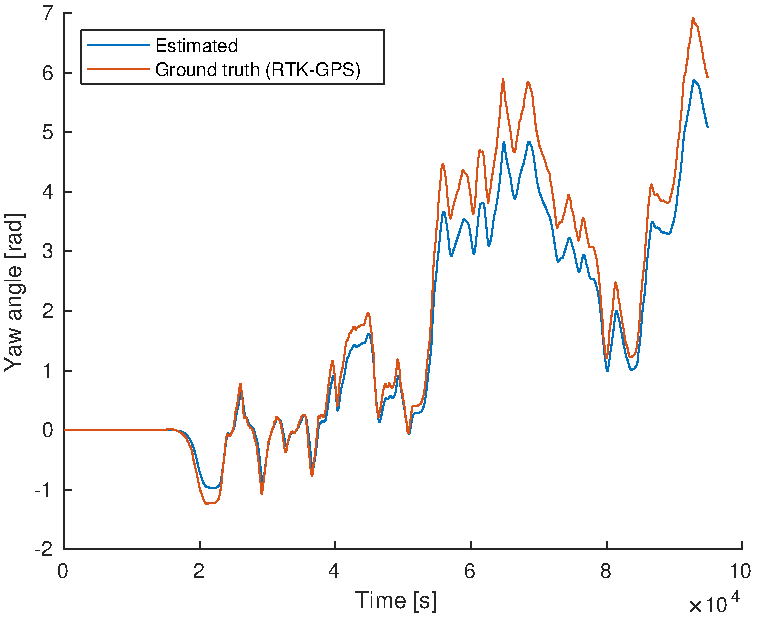
\includegraphics[width=0.8\linewidth]{0_Images/6_Results/yawFSSEndurance.pdf}
    \caption[Yaw angle while driving FSS Endurance.]
    {Yaw angle while driving FSS Endurance. Estimated compared with data from the RTK-GPS.}
    \label{Fig:YawFSSEndurance}
\end{figure}

\begin{figure}
    \centering
    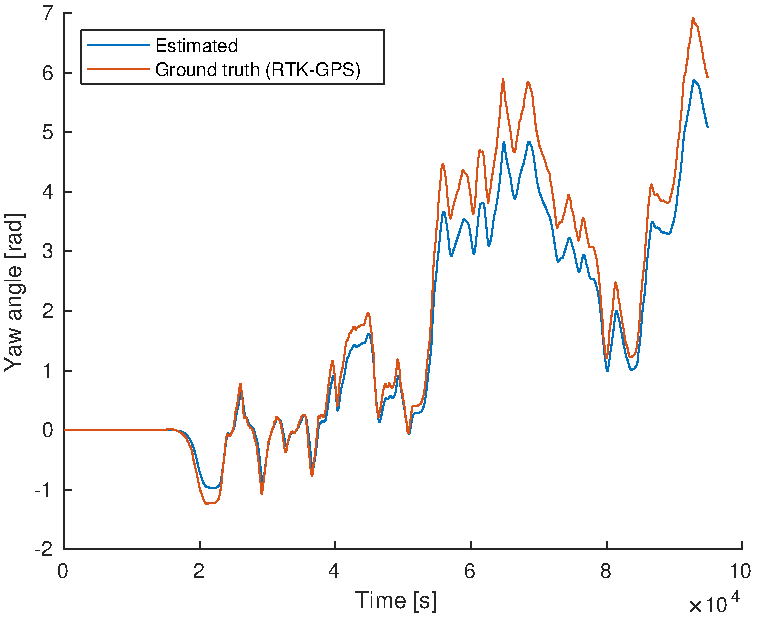
\includegraphics[width=0.8\linewidth]{0_Images/6_Results/yawFSSEndurance.pdf}
    \caption[Yaw angle while driving FSS Endurance.]
    {Yaw angle while driving FSS Endurance. Estimated compared with data from the RTK-GPS.}
    \label{Fig:YawFSSEndurance}
\end{figure}

\begin{figure}
    \centering
    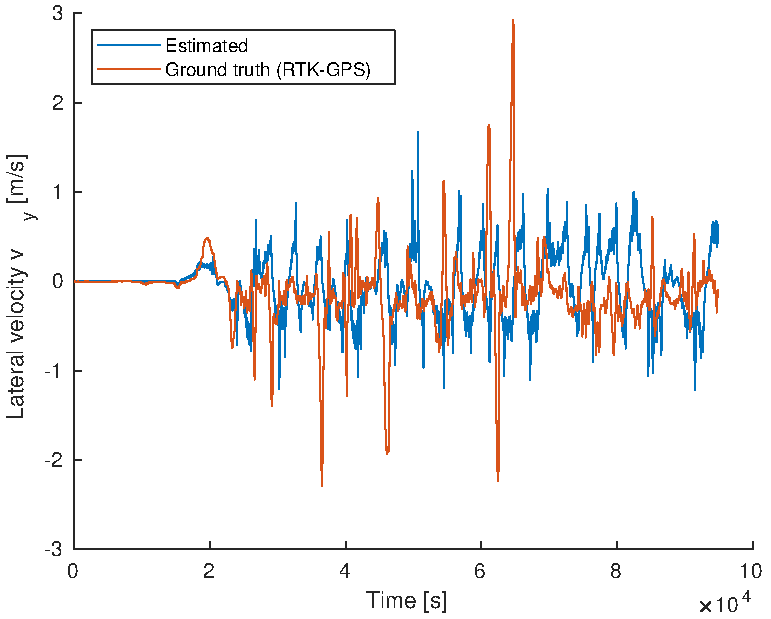
\includegraphics[width=0.8\linewidth]{0_Images/6_Results/vyFSSEndurance.pdf}
    \caption[Lateral velocity while driving FSS Endurance.]
    {Lateral velocity while driving FSS Endurance. Estimated compared with data from the RTK-GPS.}
    \label{Fig:VyFSSEndurance}
\end{figure}

\begin{figure}
    \centering
    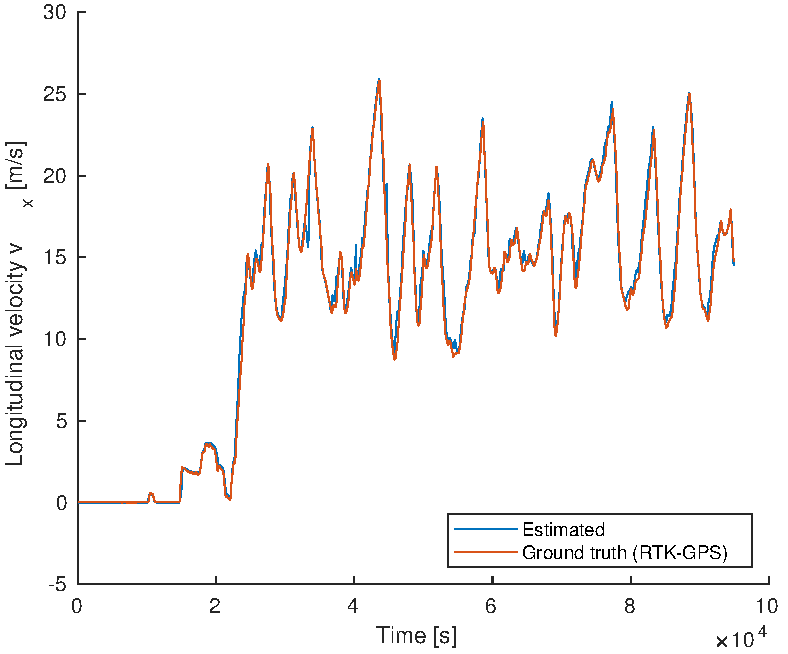
\includegraphics[width=0.8\linewidth]{0_Images/6_Results/vxFSSEndurance.pdf}
    \caption[Longitudinal velocity while driving FSS Endurance.]
    {Longitudinal velocity  while driving FSS Endurance. Estimated compared with data from the RTK-GPS.}
    \label{Fig:VxFSSEndurance}
\end{figure}

\begin{figure}
    \centering
    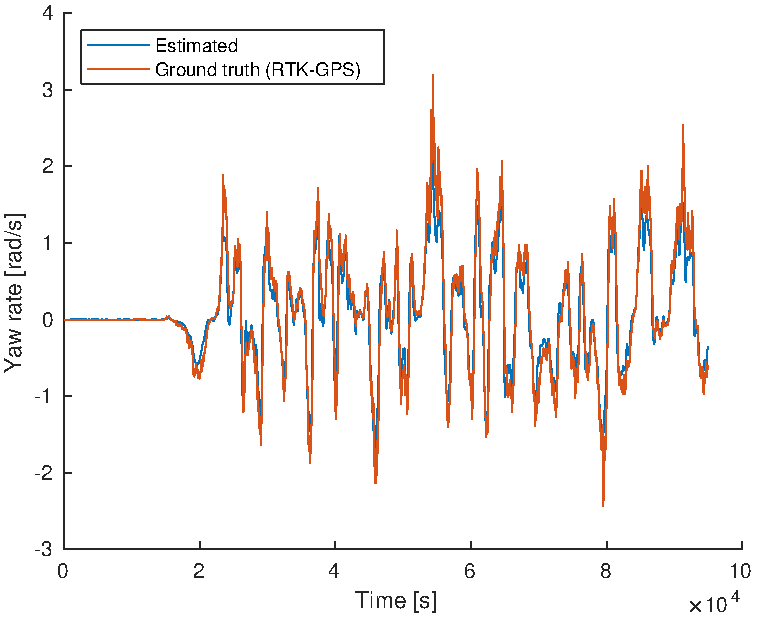
\includegraphics[width=0.8\linewidth]{0_Images/6_Results/rFSSEndurance.pdf}
    \caption[Yaw rate while driving FSS Endurance.]
    {Yaw rate  while driving FSS Endurance. Estimated compared with data from the RTK-GPS.}
    \label{Fig:RFSSEndurance}
\end{figure}

\begin{figure}
    \centering
    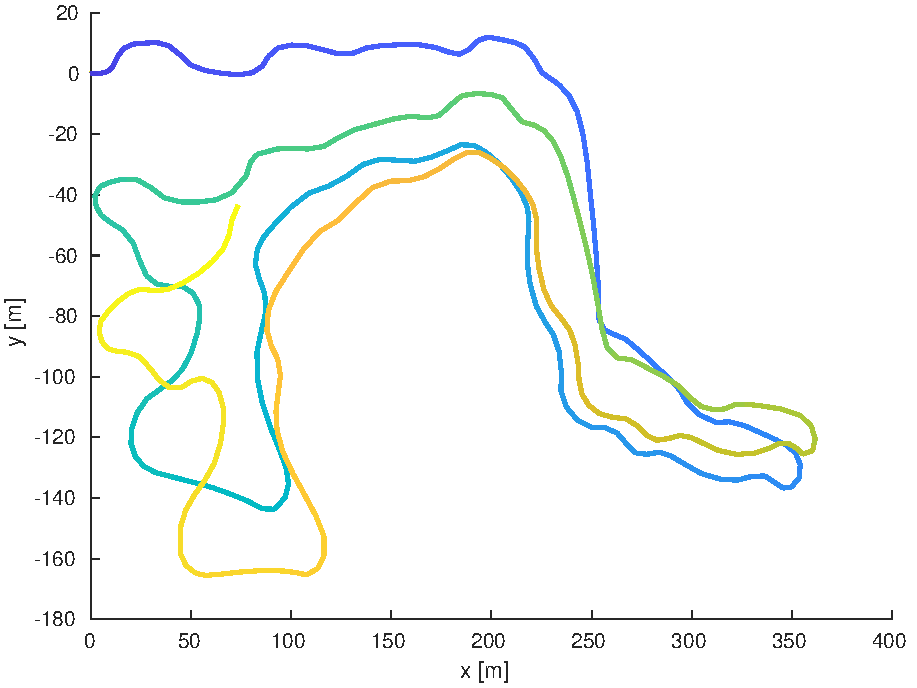
\includegraphics[width=0.8\linewidth]{0_Images/6_Results/positionFSSEndurance.pdf}
    \caption[Position while driving FSS Endurance.]
    {Position while driving FSS Endurance.}
    \label{Fig:PosFSSEndurance}
\end{figure}

\begin{figure}
    \centering
    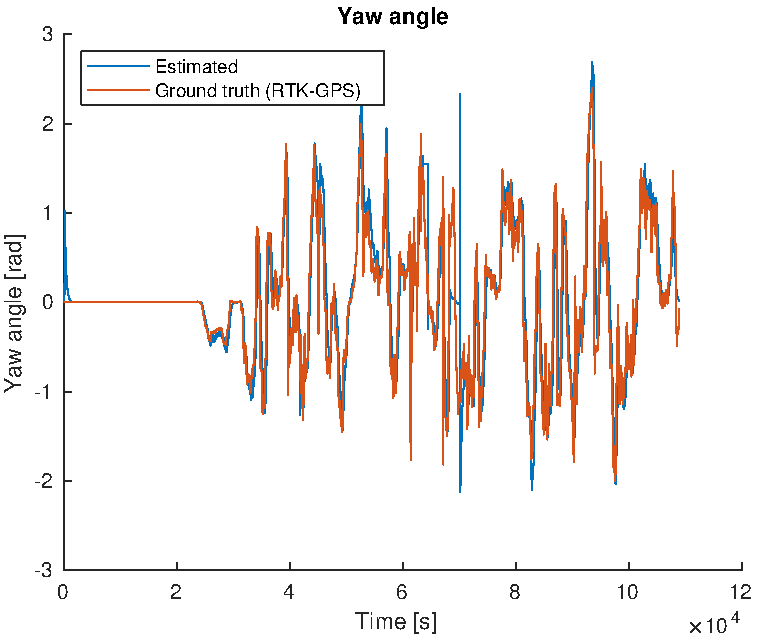
\includegraphics[width=0.8\linewidth]{0_Images/6_Results/yawFSGEndurance.pdf}
    \caption[Yaw angle while driving FSG Endurance.]
    {Yaw angle while driving FSG Endurance. Estimated compared with data from the RTK-GPS.}
    \label{Fig:YawFSGEndurance}
\end{figure}

\begin{figure}
    \centering
    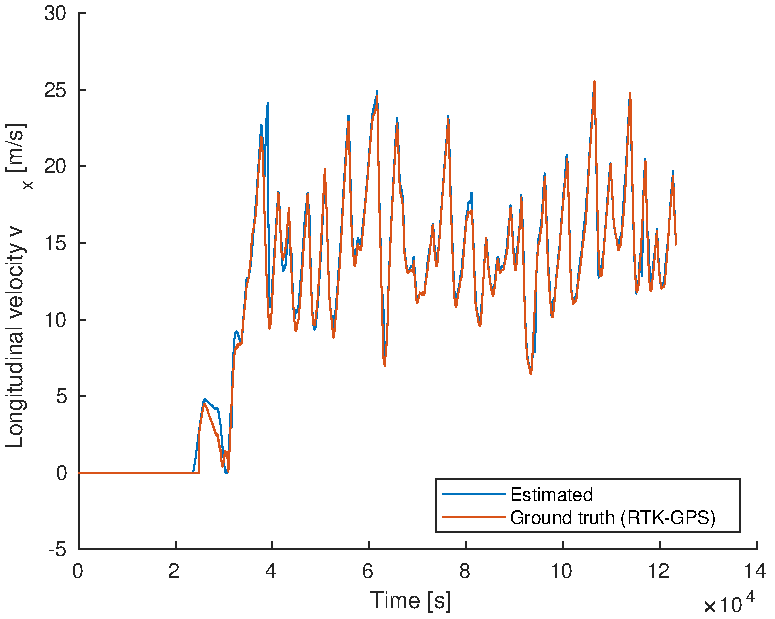
\includegraphics[width=0.8\linewidth]{0_Images/6_Results/vxFSGEndurance.pdf}
    \caption[Longitudinal velocity while driving FSG Endurance.]
    {Longitudinal while driving  during FSG Endurance. Estimated compared with data from the RTK-GPS.}
    \label{Fig:VxFSGEndurance}
\end{figure}

\begin{figure}
    \centering
    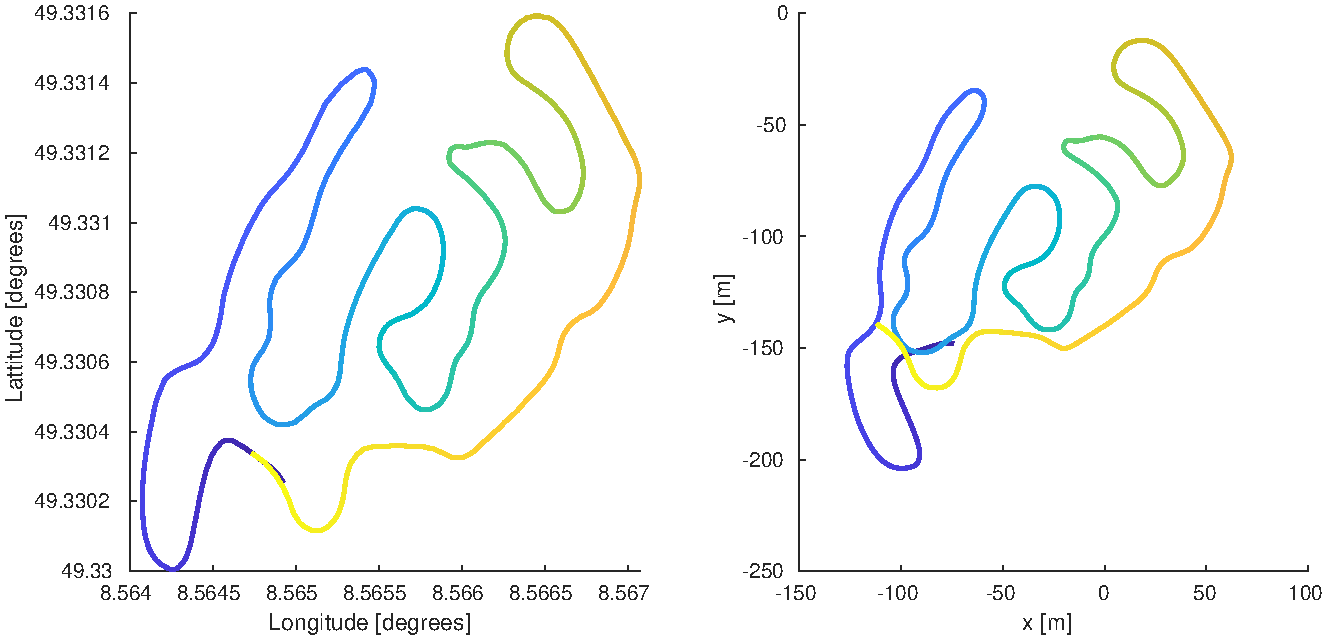
\includegraphics[width=0.8\linewidth]{0_Images/6_Results/positionFSGEndurance.pdf}
    \caption[Position while driving FSG Endurance.]
    {Position while driving FSG Endurance. Left is data from RTK-GPS while right is estimated.}
    \label{Fig:PosFSGEndurance}
\end{figure}

\begin{figure}
    \centering
    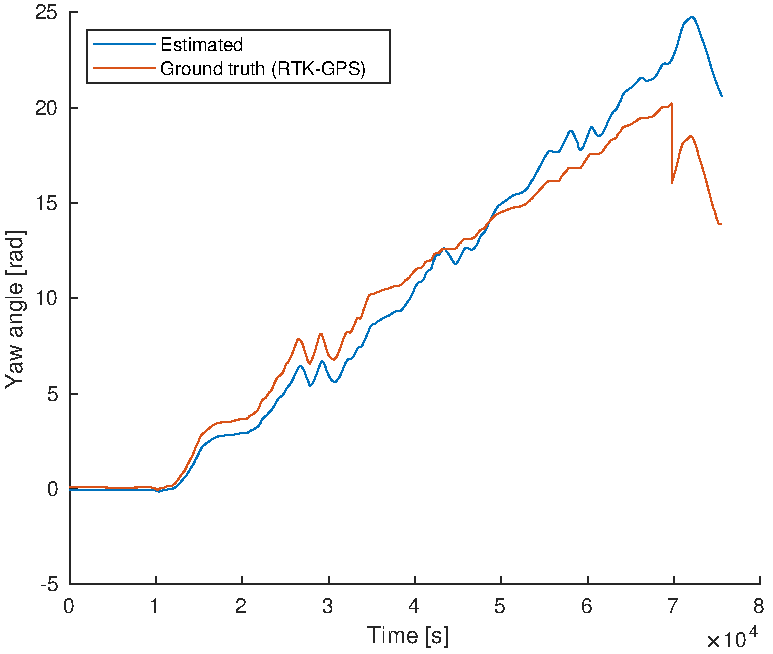
\includegraphics[width=0.8\linewidth]{0_Images/6_Results/yawFSGTestTrack.pdf}
    \caption[Yaw angle while driving FSG Test Track 1.]
    {Yaw angle while driving FSG Test Track 1. Estimated compared with data from the RTK-GPS.}
    \label{Fig:YawFSGTestTrack}
\end{figure}

\begin{figure}
    \centering
    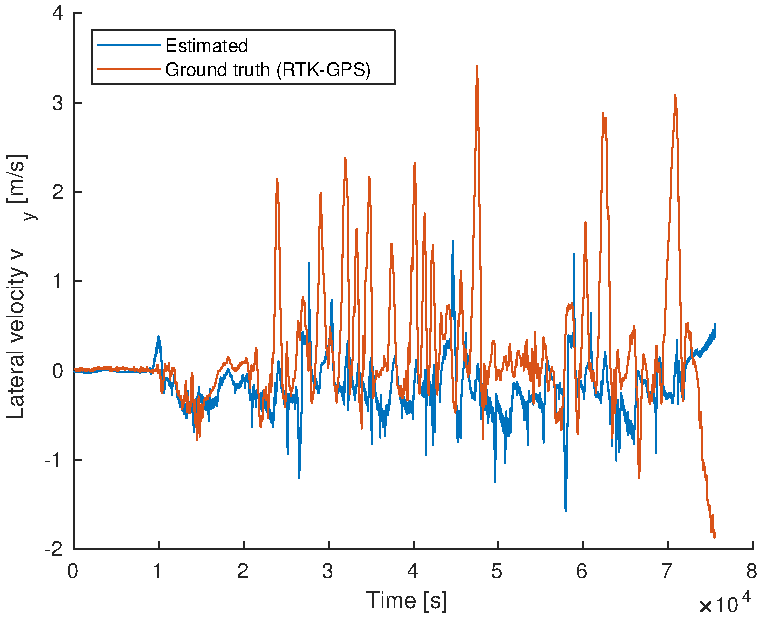
\includegraphics[width=0.8\linewidth]{0_Images/6_Results/vyFSGTestTrack.pdf}
    \caption[Lateral velocity while driving FSG Test Track 1.]
    {Lateral velocity  while driving FSG Test Track 1. Estimated compared with data from the RTK-GPS.}
    \label{Fig:VyFSGTestTrack}
\end{figure}

\begin{figure}
    \centering
    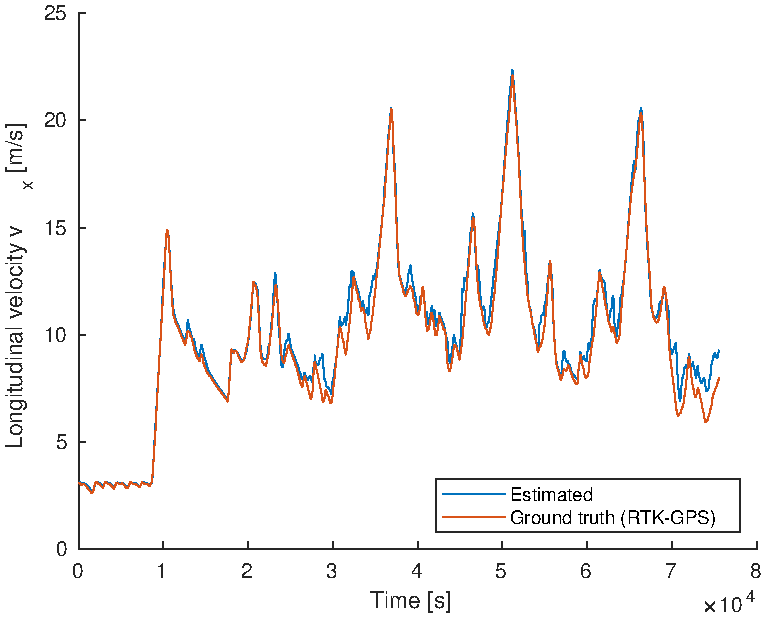
\includegraphics[width=0.8\linewidth]{0_Images/6_Results/vxFSGTestTrack.pdf}
    \caption[Longitudinal velocity while driving FSG Test Track 1.]
    {Longitudinal velocity while driving FSG Test Track 1. Estimated compared with data from the RTK-GPS.}
    \label{Fig:VxFSGTestTrack}
\end{figure}

\begin{figure}
    \centering
    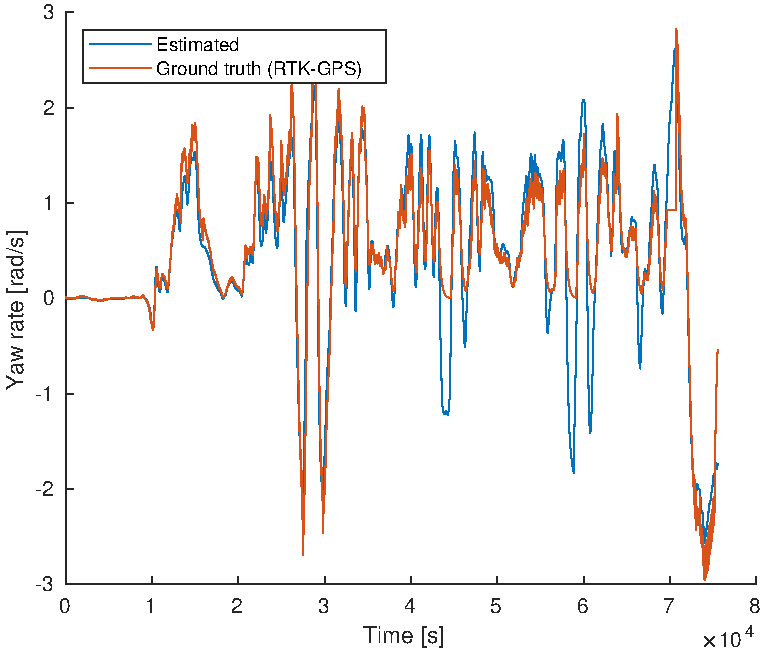
\includegraphics[width=0.8\linewidth]{0_Images/6_Results/rFSGTestTrack.pdf}
    \caption[Yaw rate while driving FSG Test Track 1.]
    {Yaw rate while driving FSG Test Track 1. Estimated compared with data from the RTK-GPS.}
    \label{Fig:RFSGTestTrack}
\end{figure}

\begin{figure}
    \centering
    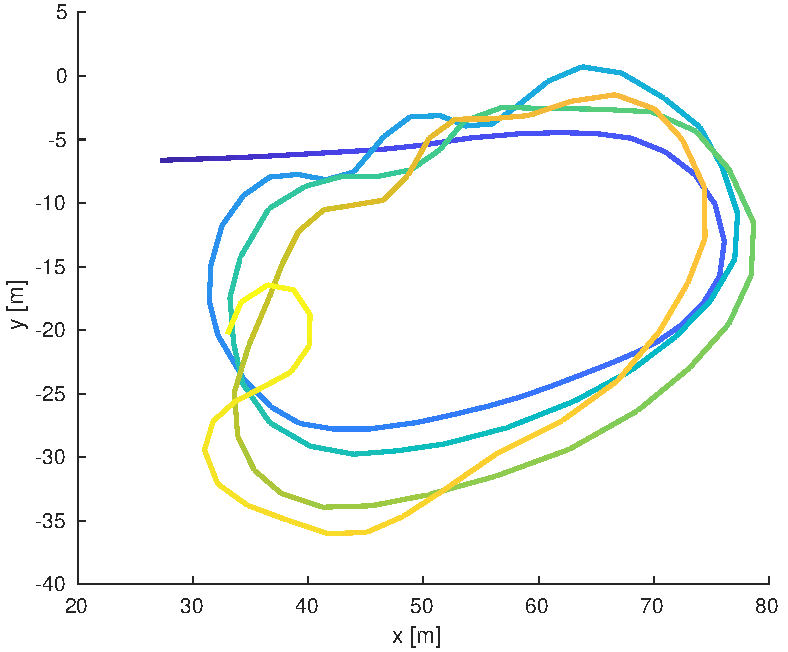
\includegraphics[width=0.8\linewidth]{0_Images/6_Results/positionFSGTestTrack.pdf}
    \caption[Position while driving FSG Test Track 1.]
    {Position while driving FSG Test Track 1.}
    \label{Fig:PosFSGTestTrack}
\end{figure}
